\documentclass[12pt]{report}
\usepackage[utf8]{inputenc}
\usepackage{authblk}
\usepackage[table]{xcolor}
\usepackage{multirow}
\usepackage{abstract}
\usepackage[font={small,it}]{caption}
\usepackage{subcaption}
\usepackage{sidecap}
\usepackage{placeins}
\usepackage{lipsum}
\usepackage{physics}
\usepackage{titlesec}
\usepackage[skins,theorems]{tcolorbox}
\tcbset{highlight math style={enhanced,
  colframe=red,colback=white,arc=0pt,boxrule=1pt}}
\usepackage[
backend=biber,
style=alphabetic,
sorting=ynt
]{biblatex}
\addbibresource{bibliography.bib}
\titleformat{\chapter}{\normalfont\huge\bfseries}{\thechapter.}{20pt}{\huge}
\renewcommand{\absnamepos}{empty}
\usepackage[
  a4paper,     
  top=25mm,
  bottom=25mm,
  width=169mm,
  bindingoffset=6mm,
  headheight=17pt, % as per the warning by fancyhdr
  heightrounded, % to avoid spurious underfull messages
]{geometry} 
\usepackage{fancyhdr,graphicx,lastpage}
\pagestyle{fancy}
\fancyhf{}
\fancyhead[L]{\rightmark} 
\fancyfoot[L, RO]{\thepage}
\fancyfoot[LO, C]{75.26 Trabajo práctico final}
\fancyfoot[CO]{Ali, Luis}
\renewcommand{\headrulewidth}{0.4pt}
\begin{document}
\begin{titlepage}
    \begin{center}
        \vspace*{1cm}
            
        \Huge
        \textbf{Simulación neuronal bajo el régimen guiado por fluctuaciones}\\
        \vspace{0.5cm}
        \LARGE
        Trabajo práctico final\\
        \vspace{1.5cm}
        \small{\emph{Autor:}\\
      	Ali Luis, \textit{Padrón Nro. 81151}\\ \texttt{aliluis@gmail.com}\\\bigskip
      	\emph{Profesores:}\\ \medskip
      	Dr. Ing. Cesar F. Caiafa\\
      	Ing. C. Marcelo Benitez\\ 
      	Lic. Azul Villanueva
      	}
            
        \vfill
            
            
        
\includegraphics[width=0.4\textwidth]{figures/logo_fiuba.png}
            
        \Large
        75.26 Simulación\\
        Departamento de computación\\
        Universidad de Buenos Aires, Fiuba
            
    \end{center}
\end{titlepage}
\thispagestyle{plain}
\begin{center}
    \Large
    \textbf{Simulación neuronal bajo el régimen guiado por fluctuaciones}
        
    \vspace{0.4cm}
    \large
    Trabajo práctico final
        
    \vspace{0.4cm}
    \small{\emph{Autor:}\\
      	Ali Luis, \textit{Padrón Nro. 81151}
      	}
       
    \vspace{0.9cm}
    \textbf{Abstract}
\end{center}
\lipsum[1]
\tableofcontents
\newpage{}
\chapter{Introducción}
\input{chapters/introducción}
\chapter{Régimen guiado por fluctuaciones}
Se analizará la media y el desvío estándar del potencial de membrana en reposo para dos modelos de neuronas. En el primero, las entradas se modelan como corrientes transitorias, mientras que en el segundo se modelan como cambios transitorios en la conductancia de membrana.
\section{Entradas modeladas como fuentes de corriente}
Se simula inyectar una corriente i(t) a través de un microelectrodo hacia el interior de la neurona.
El microelectrodo se puede pensar como una \textit{fuente de corriente ideal} y la membrana celular puede ser conceptualizada como si estuviera hecha por varios circuitos RC (ver figura~\ref{fig:modelo_neurona_esferica}). Como las dimensiones de la célula son muy pequeñas, el potencial en la superficie de la membrana es el mismo en todos lados. De esta manera, el comportamiento eléctrico de la célula puede ser descrito adecuadamente por un único circuito RC con una fuente de corriente (ver figura~\ref{fig:circuito_electrico_integrate_and_fire_potencial_reposo}).
\begin{figure*}[htbp!]
        \centering
        \begin{subfigure}[b]{0.45\textwidth}  
            \centering 
            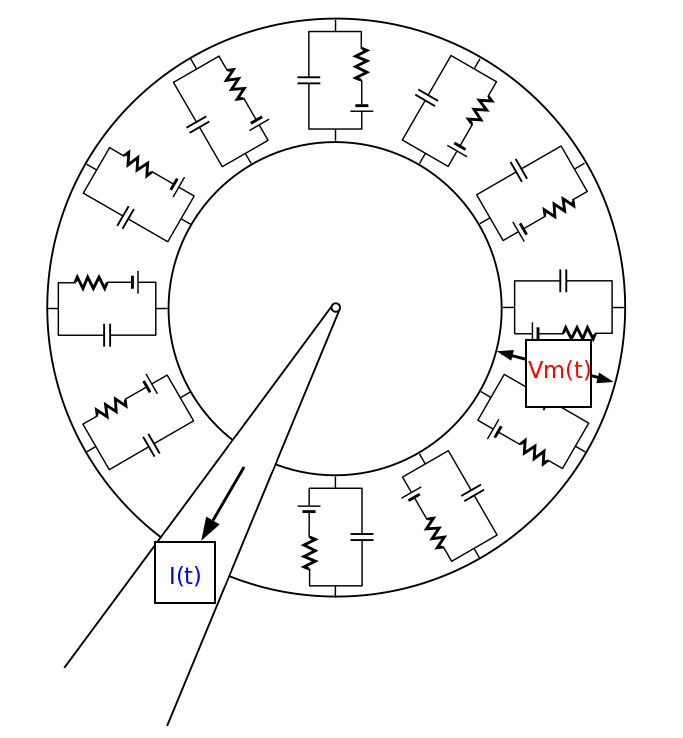
\includegraphics[width=6cm]{figures/neurona_esferica_conceptual.png}
            \caption{Modelo eléctrico de una célula esférica. Por convención, una corriente saliente es positiva, por ese motivo la flecha se dibuja así.}
            \label{fig:modelo_neurona_esferica}
        \end{subfigure}
         \hspace{0.5cm}
        \begin{subfigure}[b]{0.45\textwidth}
            \centering
            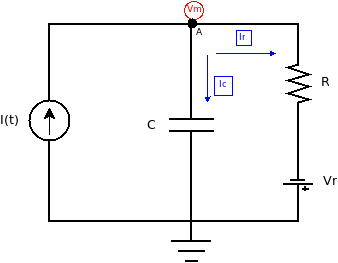
\includegraphics[width=\textwidth]{figures/integrate_fire_con_potencial_reposo.png}
            \caption{Circuito eléctrico que representa una pequeña porción de membrana. La corriente $I_r$ también es conocida como la corriente de fuga $I_l$.}
            \label{fig:circuito_electrico_integrate_and_fire_potencial_reposo}
        \end{subfigure}
        \quad
        \caption{Estructura eléctrica de una neurona}
        \label{fig:estructura_electrica_neurona}
\end{figure*}
\newpage
Siguiendo un desarrollo similar al de la sección~\ref{sec:modelo_leaky_integrate_and_fire}, pero esta vez teniendo en cuenta el potencial de reposo, la corriente que circula a través de la resistencia es:
\begin{equation}\label{eq:corriente_resistencia_fuga}
    \boxed{i_r(t)= \frac{v_m(t)-v_r}{R}}    
\end{equation}
De esta manera, se obtiene\cite{Kuhn2345}:
\begin{equation}\label{eq:ecuacion_diferncial_koch}
    \tcbhighmath[boxrule=1pt,arc=1pt,colback=blue!10!white,colframe=black]{\tau_m \dv{v_m}{t} = -\big[v_m(t) - v_r\big] + \frac{i(t)}{g_l},\ con\ v_m(0)= v_r}
\end{equation}
\begin{center}
\begin{tabular}{ r l}
\footnotesize{donde,}&\\
 \footnotesize{$v_m(t)$:}& \footnotesize{es el potencial de membrana}\\ 
 \footnotesize{i(t)}:& \footnotesize{corriente de entrada.}\\
 \footnotesize{C:}& \footnotesize{capacitancia de membrana}\\
 \footnotesize{$g_l$}:& \footnotesize{conductancia de fuga (leak)}\\
 \footnotesize{$v_r$:}& \footnotesize{potencial de reposo}
\end{tabular}
\end{center}
\subsubsection{Corriente de entrada i(t)}
La corriente i(t) es inducida por eventos sinapticos excitatorios (CEPS-Corriente excitatoria postsinaptica) e inhibitorios (CEPS - corriente inhibitoria postsinaptica) (ver sección \ref{sec:sinapsis_quimica}):
\begin{equation}
    i(t)= i_e(t) + i_i(t)=\sum_j CEPS(t-t_j) + \sum_k CIPS(t-t_k)
\end{equation}
donde, $t_j\ y\ t_k$ son los tiempos de ocurrencia de los eventos excitatorios e inhibitorios respectivamente. Se asume que estos tiempos de ocurrencia siguen una distribución Poisson:
\[t_j\sim Poi\big(\lambda_e\big) \]
\[t_k\sim Poi\big(\lambda_i\big) \]
Una CEPS y una CIPS individual se modela como funciones $\alpha$ \cite{10.5555/1137840}:
\[
    \tcbhighmath[fuzzy halo=1mm with blue!50!white,arc=2pt,
  boxrule=0pt,frame hidden]{CEPS(t)=A_e \frac{t}{\tau_e}e^{(1-t/\tau_e)}H(t)}
\]
\[
    \tcbhighmath[fuzzy halo=1mm with blue!50!white,arc=2pt,
  boxrule=0pt,frame hidden]{CIPS(t)=A_i \frac{t}{\tau_i}e^{(1-t/\tau_i)}H(t)}
\]
\begin{center}
\begin{tabular}{ r l}
 $A_e>0,\ A_i<0$:& corrientes pico\\ 
 $\tau_e,\ \tau_i$:& constantes de tiempo.
\end{tabular}
\end{center}
H(x) es la \textit{función escalón Heaviside}
\begin{equation}\label{eq:heaviside}
    H(x)= \begin{cases} 
      0 & x< 0 \\
      1 & x \geq 0 
   \end{cases}
\end{equation}
Como el sistema definido por la ecuación~\ref{eq:ecuacion_diferncial_koch} es \textit{lineal}, alcanza con conocer la respuesta de la membrana a una única corriente postsinaptica (CPS) para inferir las propiedades estadísticas causadas por múltiples CPS (bombardeo sinaptico). La respuesta a una única CPS está dada por la solución del sistema de la ecuación~\ref{eq:ecuacion_diferncial_koch} tomando i(t)=CPS(t), donde CPS(t) puede ser tanto CEPS(t) como CIPS(t).
\[
    \tcbhighmath[fuzzy halo=1mm with blue!50!white,arc=2pt,
  boxrule=0pt,frame hidden]{CPS(t)=\frac{A_s.e}{C.\tau_s}.\Bigg[\frac{-t.e^{-\frac{t}{\tau_s}}}{\frac{1}{\tau_s}-\frac{1}{\tau_m}}+\frac{e^{-\frac{t}{\tau_m}}-e^{-\frac{t}{\tau_s}}}{\big(\frac{1}{\tau_s}-\frac{1}{\tau_m}\big)^2}\Bigg].H(t)}
\]
El par $(A_s,\ \tau_s)$ puede ser tanto $(A_e,\ \tau_e)$ como $(A_i,\ \tau_i)$ \\
Como el bombardeo de potenciales de acción sigue una distribución Poisson y varias CPS se suman de manera lineal, la media $\mu(v_m)$ y la varianza $\sigma^2(v_m)$ del potencial de membrana está dado por el teorema de Campbell \cite{papoulis1991probability}:
\begin{equation}
    \tcbhighmath[boxrule=1pt,arc=1pt,colback=blue!10!white,colframe=black]{\mu(v_m)=v_r+\int CEPS(t) dt+ \lambda_i.\int CIPS(t) dt}
\end{equation}
\begin{equation}
    \tcbhighmath[boxrule=1pt,arc=1pt,colback=blue!10!white,colframe=black]{
    \sigma^2(v_m)=\lambda_e.\int CEPS^2(t) dt + \lambda_i.\int CIPS^2(t) dt
    }
\end{equation}
donde:
\[
    \tcbhighmath[fuzzy halo=1mm with blue!50!white,arc=2pt,
  boxrule=0pt,frame hidden]{\int CPS(t)dt= \frac{A_s.\tau_s.e.\tau_m}{C}}
  \]
 \[
    \tcbhighmath[fuzzy halo=1mm with blue!50!white,arc=2pt,
  boxrule=0pt,frame hidden]{\int CPS^2(t)dt= (2.\tau_m + \tau_s).\Bigg[\frac{A_s.\tau_s.e.\tau_m}{2C(\tau_m+\tau_s)}\Bigg]^2}
  \]
  
\appendix
\chapter{Biología de la neurona}
Las neuronas se comunican entre sí mediante la \textit{sinápsis} (ver el sitio web \cite{khanacademywebsite}). La \textit{sinápsis} es el punto de comunicación entre dos neuronas, o entre una neurona y una glándula. En la sinápsis, el disparo de un \textit{potencial de acción} en una neurona (la neurona \textbf{presináptica} o emisora), provoca la transmisión de una señal a otra neurona (la neurona \textbf{postsináptica} o receptora), lo que aumenta o disminuye la probabilidad de que la neurona postsináptica dispare su propio \textit{potencial de acción} (ver figura~\ref{fig:Sinapsis}). 
\begin{figure}[htbp!]
    \centering
    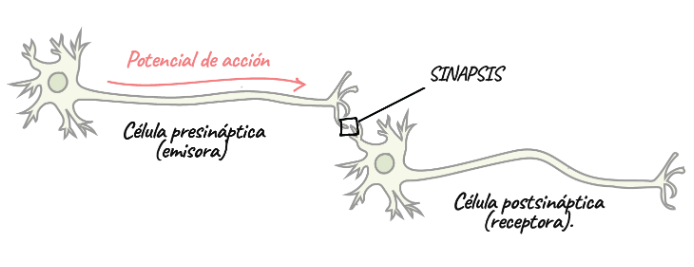
\includegraphics[width=10.0cm]{figures/Sinapsis.png}
    \caption{Sinápsis. Comunicación entre neuronas}
    \label{fig:Sinapsis}
\end{figure}
\section{Potencial de membrana}\label{section:Potencial_Membrana}
Las neuronas tienen, además del potencial de acción, un \textit{potencial de reposo} (potencial de membrana en reposo) (ver  el sitio web \cite{khanacademywebsite}). Si uno pudiera tomar las puntas de un voltímetro y colocarlas una en el exterior y otra en el interior de la membrana plasmática de una célula viva, se mediría una diferencia de potencial o voltaje al que se denomina \textbf{potencial de membrana}. El punto de referencia es el exterior de la célula. En la mayoría de las neuronas en reposo, la diferencia de potencial de la membrana es de 30 mV a 90 mV, con el interior de la célula más negativo que el exterior. Es decir, las neuronas tienen un \textbf{potencial de membrana en reposo} de -30 mV a -90 mV.
\begin{figure}[htbp!]
    \centering
    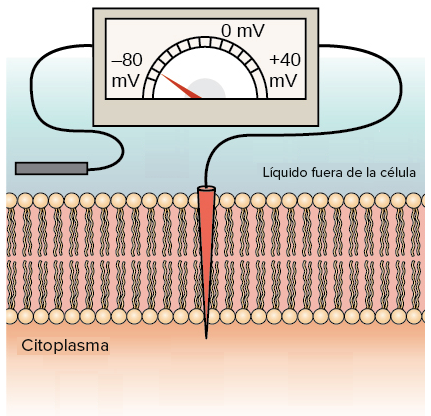
\includegraphics[width=4.5cm]{figures/potencial_membrana.png}
    \caption{Potencial de membrana}
    \label{fig:Potencial_membrana}
\end{figure}
El potencial de reposo de membrana está determinado por la distribución desigual de \textbf{iones} entre el interior y el exterior de la célula, y por las diferencias en la permeabilidad de la membrana hacia diferentes tipos de iones. En las neuronas y sus líquido circundante, los iones más abundantes son:
\begin{itemize}
    \item Cationes (iones con carga positiva): Sodio ($Na^+$) y potasio ($K^+$)
    \item Aniones (iones con carga negativa): Cloruro ($Cl^-$) y aniones orgánicos (proteínas y aminoácidos)
\end{itemize}
\newpage
En la mayoría de las neuronas, el $k^+$ y los aniones orgánicos se encuentran en concentraciones más altas dentro que fuera de la célula. En cambio, el $Na^+$ y el $Cl^-$ generalmente se encuentran en concentraciones más altas fuera de la célula (fig.~\ref{fig:concentracion_iones}). Esto significa que a través de la membrana existe un gradiente de concentración por la acumulación de partículas en mayor cantidad en un lado que en otro. Las partículas se difunden a favor del gradiente de concentración desde áreas de mayor concentración hacia áreas de menor concentración, hasta que estén igualmente distribuidas.
\begin{figure*}[h!]
        \centering
        \begin{subfigure}[b]{0.35\textwidth}
            \centering
            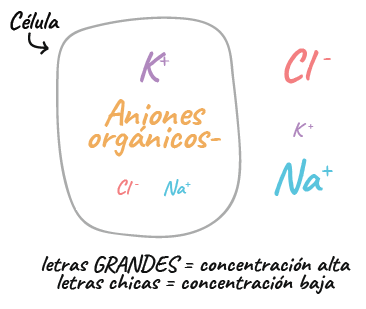
\includegraphics[width=\textwidth]{figures/concentracion_iones.png}
            \caption{Concentración de iones dentro y fuera de la célula}
            \label{fig:concentracion_iones}
        \end{subfigure}
        \hspace{1.5cm}
        \begin{subfigure}[b]{0.4\textwidth}  
            \centering 
            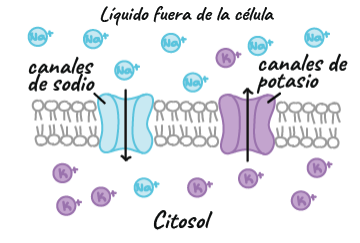
\includegraphics[width=\textwidth]{figures/canales_iones.png}
            \caption{Canales a través de los cuales los iones cruzan la membrana}
            \label{fig:canales_iones}
        \end{subfigure}
        \quad
        \caption{Concentración de iones y movimiento dentro y fuera de la célula}
\end{figure*}
Debido a su carga, los iones no pueden pasar directamente a través de las regiones de lípidos hidrofóbicos ("temerosos del agua") de la membrana, sino que lo tienen que hacer a través de \textit{canales de proteínas} especializados que proporcionan un túnel hidrofílico ("amigo del agua") que cruzan la membrana. Existen canales, llamados \textit{canales de filtración}, que están abiertos en membranas en reposo y canales que se cierran en neuronas en reposo y sólo se abren en respuesta a una señal.\\
Los canales iónicos que permiten solamente el paso de $k^+$ se llaman \textbf{canales de potasio} y los que permiten principalmente el paso del $Na^+$ se denominan \textbf{canales de sodio} (fig.~\ref{fig:canales_iones}).\\
El movimiento de iones $k^+$ a través de la membrana es el principal responsable del potencial de membrana de una neurona en reposo. Cuando hay una mayor concentración de $k^+$ dentro de la célula que en el líquido circundante y se abren los canales de potasio en la membrana, el $k^+$ comenzará a fluir por su gradiente de concentración hacia el exterior de la célula. Cada vez que un ión $k^+$ sale de la célula, el interior de la célula pierda una carga positiva. En el exterior de la membrana celular se acumula un ligero exceso de carga positiva y en el interior se acumula un ligero exceso de carga negativa. El interior de la célula se vuelve negativo a comparación del exterior y se establece una diferencia de potencial eléctrico en la membrana.\\
Cuando se establece la diferencia de potencial eléctrico en la membrana se dificulta que los iones $k+$ restantes puedan salir de la célula debido a que los iones $k^+$ de carga positiva son atraídos por los iones de carga negativa del interior de la célula y a su vez son repelidos por las cargas positivas del exterior. Todo esto se opone al movimiento en dirección del gradiente de concentración.\\
La diferencia de potencial en la membrana se acumula hasta que la \textit{fuerza eléctrica} que impulsa al $k^+$ de regreso a la célula sea igual a la \textit{fuerza química} que impulsa la salida del $k^+$ a través de los canales. En ese punto, no hay movimiento neto de $k^+$ y el sistema entra en equilibrio. Cada vez que un $k^+$ sale de la célula, otro $k^+$ entrará en ella.\\
La diferencia de potencial eléctrico en la membrana celular que equilibra exactamente con el gradiente de concentración de un ion se conoce como \textbf{potencial de equilibrio} (El potencial de equilibrio de un ion depende de la concentración de ese ion). Si el gradiente de concentración es muy intenso, el potencial eléctrico que lo equilibra debe ser muy grande.
La mayoría de las neuronas en reposo son permeables al $Na^+$ y al $Cl^-$ asi como al $k^+$. En particular, la permeabilidad del potasio es la principal razón por la que su potencial de membrana en reposo es diferente al potencial de equilibrio del potasio.\\
Si se toma un modelo de membrana permeable con el $Na^+$ como único ion (en lugar del potasio) que puede cruzar la membrana, el $Na^+$ generalmente está más concentrado afuera de la célula, por lo que se moverá en el sentido del gradiente de concentración hacia la célula volviendo más positivo el interior de la misma que el exterior. Debido a esto, el potencial de equilibrio del sodio será positivo y en un sistema donde $Na^+$ es el único ion permeante, el potencial de membrana será positivo.\\
En una neurona en reposo, el $Na^+$ y el $k^+$ son permeantes, o capaces de atravesar la membrana.
\begin{itemize}
    \item El $Na^+$ intentará arrastrar el potencial de membrana hacia su potencial de equilibrio (positivo)
    \item El $k^+$ intentará arrastrar el potencial de membrana hacia su potencial de equilibrio (negativo)
\end{itemize}
El potencial de membrana real estará entre el punto de equilibrio del $Na^+$ y entre el punto de equilibrio del $k^+$. Sin embargo, será \textit{más cercano} al potencial de equilibrio del ion más permeable (el que atraviese la membrana con más facilidad).\\
En una neurona, el potencial de membrana estará más cerca del potencial de equilibrio del $k^+$ que del $Na^+$ porque el $k^+$ es mucho más permeable que el $Na^+$.
\begin{itemize}
    \item Si se abrieran más canales de potasio, le membrana se \texttt{hiperpolarizaría} y se acercaría todavía más al potencial de equilibrio del potasio.
    \item Si se abrieran más canales de sodio, le membrana se \texttt{despolarizaría} hacia al potencial de equilibrio del sodio.
\end{itemize}
Cambiar el número de canales abiertos proporciona una forma de controlar el potencial de membrana de la célula y es una forma muy importante de producir \textit{señales eléctricas}
\newpage
\section{Bomba Sodio-Potasio}\label{sec:bomba_sodio_potasio}
La \textit{bomba sodio-potasio} es una enzima que realiza un transporte bombeando iones sodio afuera hacia afuera de la célula y al mismo tiempo bombea iones de potasio desde el exterior hacia el interior celular. Esta bomba es responsable de mantener las diferencias de concentración de sodio y de potasio a través de la membrana celular, así como de establecer un voltaje eléctrico negativo en el interior de las células. Se encuentra en la membrana plasmática de todas las células animales.\\
La bomba expulsa tres iones sodio ($Na^+$) hacia la matriz extracelular a la vez que ingresa dos iones potasio ($k^+$) hacia el citoplasma mediante transporte activo que ocupa como fuente de energía el ATP\footnote{\footnotesize El \textbf{trifosfato de adenosina} sirve para la obtención de energía celular. Se produce durante la respiración celular y es consumido por muchas enzimas en la catálisis de numerosos procesos químicos.}. Este bombeo permanente permite mantener el gradiente electroquímico de solutos con una concentración elevada de potasio dentro de la célula y bajo afuera, mientras que la concentración de sodio es baja dentro de la célula y elevada afuera. Este proceso es responsable de mantener el gran exceso de $Na^+$ afuera de la célula y el gran exceso de $k^+$ en el interior de la célula.
\begin{figure}[htbp!]
    \centering
    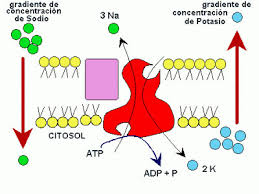
\includegraphics[width=7.5cm]{figures/bomba_sodio.jpeg}
    \caption{Bomba sodio-potasio}
    \label{fig:bomba_sodio_potasio}
\end{figure}
\section{Potencial de acción}
\begin{figure*}[htbp!]
        \centering
        \begin{subfigure}[b]{0.4\textwidth}
            \centering
            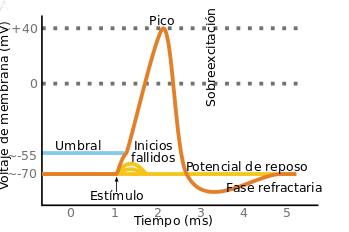
\includegraphics[width=\textwidth]{figures/potencial_accion_esquematico.png}
            \caption{Vista esquemática de un potencial de acción ideal, mostrando las distintas fases}
            \label{fig:potencial_accion_ideal}
        \end{subfigure}
        \hspace{1.25cm}
        \begin{subfigure}[b]{0.4\textwidth}  
            \centering 
            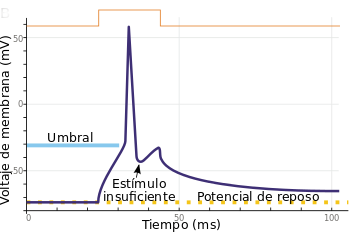
\includegraphics[width=\textwidth]{figures/potencial_accion_real.png}
            \caption{Registro real de un potencial de acción}
            \label{fig:potencial_accion_real}
        \end{subfigure}
        \quad
        \caption{Potencial de acción}
        \label{fig:potencial_accion}
\end{figure*}
Cuando se aplica a una neurona un estímulo de intensidad suficiente para que el potencial de membrana alcance un límite denominado \textbf{umbral}, se genera una señal que recibe el nombre de \textbf{potencial de acción} (ver sitio web \cite{khanacademywebsite}).
Un potencial de acción es un cambio muy rápido en la polaridad de la membrana de negativo a positivo y de vuelta a negativo, en un ciclo que dura unos milisegundos. Cada ciclo comprende una \textit{fase ascendente}, una\textit{ fase descendente} y una \textit{fase hiperpolarizada}.\\
El potencial de acción no se mantiene en un punto de la membrana plasmática, sino que viaja a lo largo de la membrana. Puede desplazarse a lo largo de un axón a mucha distancia.
\newpage
\subsection{Fases del potencial de acción}\label{subsec:fases_potencial_accion}
\begin{enumerate}
\item \textbf{Fase ascendente}: El estímulo que se aplica a una neurona es una despolarización lo suficientemente grande que aumente el voltaje de la membrana y cruce el valor del umbral (generalmente de -55 mV). Cuando el estímulo llega al umbral, provoca que  se abran los canales de $Na^+$ dependientes del voltaje en la membrana, lo cual permite que ingresen varios iones de sodio precipitadamente a la célula. Estos iones de sodio hace que aumente muy rápido el potencial de membrana hasta +40 mV. En el pico del potencial, el potencial de membrana se encuentra cerca del potencial de equilibrio del sodio.
\item \textbf{Fase descendente}: Cuando el potencial llega al pico, el mismo voltaje del estímulo que provocó la apertura de los canales de sodio al alcanzar el umbral, ahora genera el cierre gradual\footnote{\footnotesize El tiempo que transcurre hasta dejar inactivo a los canales de sodio luego del pico, es muy breve. Prácticamente quedan inactivos en el pico.} de los mismos hasta dejarlos inactivos\footnote{\footnotesize Estado inactivo: Deja de circular iones desde o hacia el interior de la célula}. Al mismo tiempo, el voltaje del estímulo abre los canales de potasio, permitiendo que el potasio salga precipitadamente de la célula. El incremento de la permeabilidad del potasio lleva al potencial de membrana cerca del potencial de equilibrio del potasio. El efecto combinado de los cambios en la permeabilidad del sodio y del potasio hacen que el potencial de membrana caiga rápidamente, repolarizando la membrana y generando una \textit{fase descendente} del potencial de acción.
\item \textbf{Fase hiperpolarizada}: El voltaje despolarizado abre canales de potasio adicionales y algunos de estos no se cierran cuando el potencial de membrana vuelve a su potencial de reposo, además se abrieron canales de potasio adicionales en respuesta a la entrada de iones de sodio durante el potencial de acción. La concentración de $k^+$ en el interior de la célula es inusualmente baja, haciendo que el potencial de membrana se acerque mucho más al potencial de equilibrio del potasio. El potencial de membrana va por debajo del potencial de reposo lo cual produce una \textit{hiperpolarización} que persiste hasta que la permeabilidad del potasio regresa a su estado norma. Los canales de potasio se cierran gradualmente, haciendo que se restaure el potencial de membrana hacia el valor del potencial de reposo. Los canales de sodio vuelven a su estado normal \footnote{\footnotesize Estado normal de  los canales de sodio: Permanecen cerrados pero pueden responder al voltaje}.
\end{enumerate}
\subsection{Período refractario}\label{subsec:periodo_refractario}
El tiempo durante el cual es imposible o difícil generar un segundo potencial de acción luego de haber generado uno anteriormente, es el período refractario. Este período se puede superponer con otras fases del potencial de acción.\\
Cada potencial de acción es seguido por un período refractario que puede ser dividido en \textit{período refractario absoluto} y \textit{período refractario relativo}. Estos dos períodos refractarios son debido al cambio de estado de los canales de sodio y potasio.
\begin{itemize}
    \item \textbf{Período refractario absoluto}: Durante este período es imposible generar un potencial de acción. Cuando los canales de sodio quedan inactivos luego del potencial de acción, no se pueden abrir, sin importar cual sea el potencial de membrana porque entran en un estado \textit{inactivo}.
    \item \textbf{Período refractario relativo}: Este período comprende el breve tiempo luego del período refractario absoluto, cuando algunos canales de sodio ya se recuperaron de su inactivación y pueden desencadenar un segundo potencial de acción, de menor amplitud porque hay menos canales de sodio activos y además requiere un estímulo mayor para poder llegar al umbral.
\end{itemize}
\section{Sinapsis química}\label{sec:sinapsis_quimica}
Un sólo axón puede tener múltiples ramificaciones, lo que le permite hacer sinápsis con una o varias células postsinápticas. Del mismo modo, una neurona puede recibir miles de entradas sinápticas de muchas neuronas presinápticas o emisoras diferentes.\\
Dentro de la terminal axónica emisora hay muchas \textit{vescículas sinápticas}. Son esferas membranosas llenas de moléculas de \textit{neurotrasnmisor}. El pequeño espacio entre la terminal axónica de la neurona presináptica y de la membrana de la célula postsináptica se llama \textbf{espacio sináptico}.
\begin{figure*}[h!]
        \centering
        \begin{subfigure}[b]{0.475\textwidth}
            \centering
            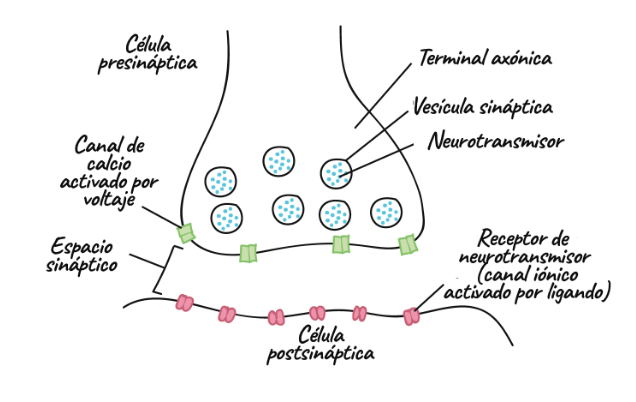
\includegraphics[width=\textwidth]{figures/conexion_neuronas.png}
            \caption{Anatomía de la conexión entre células}
            \label{fig:anatomia_conexion}
        \end{subfigure}
        \hfill
        \begin{subfigure}[b]{0.475\textwidth}  
            \centering 
            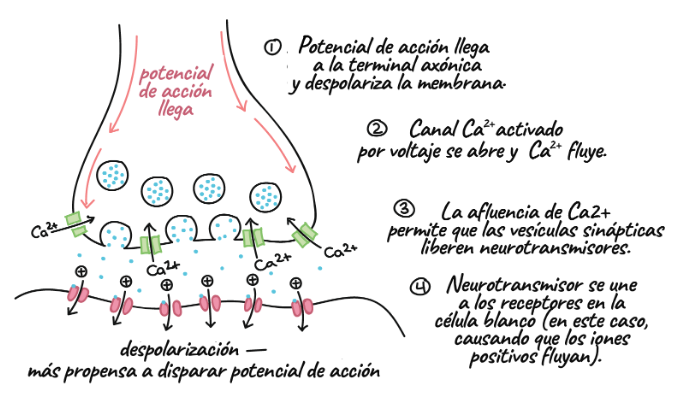
\includegraphics[width=\textwidth]{figures/neurotransmisores.png}
            \caption{Neurotransmisores viajando desde una neurona a otra a través del espacio sináptico}
            \label{fig:neurotransmisores}
        \end{subfigure}
        \quad
        \caption{Conexión entre neuronas}
        \label{fig:conexion_neuronas}
\end{figure*}
Existen muchas \textbf{vescículas sinápticas} dentro de la terminal axónica de una célula emisora (ver figura~\ref{fig:anatomia_conexion}). Son esferas membranosas llenas de moléculas de neurotransmisores. El pequeño espacio entre la terminal axónica de la neurona presináptica y la membrana de la célula postsináptica se llama \textbf{espacio sináptico}.\\
La figura~\ref{fig:neurotransmisores} muestra que cuando llega un potencial de acción o impulso nervioso a la terminal axónica, acciona canales de calcio activados por voltaje en la membrana celular. \newpage
El $Ca^{2+}$ que está muchos más concentrado afuera de la neurona que adentro, entra a la célula. El $Ca^{2+}$ permite que las vescículas sinápticas se fundan con la membrana de la terminal axónica haciendo que se liberen los neurotransmisores en el espacio sináptico. Las moléculas del neurotrasnmisor se difunden por el espacio sináptico y se unen a las proteínas receptoras en la célula postsináptica.\\
Cuando un neurotransmisor se une a su receptor en la célula receptora, causa la apertura o cierre de canales iónicos. Esto puede producir un cambio localizado en el potencial de membrana de la célula receptora.
\begin{itemize}
    \item En algunos casos provoca que la célula sea más propensa a disparar su propio potencial de acción. En este caso el cambio en el potencial de membrana se llama \textbf{potencial excitatorio postsináptico} o \textbf{PEPS}
    \item En otros casos provoca que la célula sea menos propensa a disparar su propio potencial de acción y se llama \textbf{potencial inhibitorio postsináptico} o \textbf{PIPS}
\end{itemize}
Un PEPS es despolarizante: hace que el interior de la célula sea más positivo y acerca el potencial de membrana a su umbral de disparo de un potencial de acción. A veces no es suficiente un PEPS aislado para llevar a la neurona al umbral, pero puede sumarse junto con otros PEPS para desencadenar un potencial de acción.
Los PIPS tienen el efecto contrario. Tienden a mantener el potencial de membrana de la neurona postsináptica por debajo del umbral del potencial de acción. Los PIPS pueden contrarrestar o cancelar el efecto excitatorio de los PEPS.\\
Una neurona postsináptica suma o integra todas las señales inhibitorias y excitatorias que recibe y "decide" si quiere disparar o no un potencial de acción.
\begin{itemize}
    \item La integración de potenciales postsinápticos que ocurren en diferentes lugares pero casi al mismo tiempo se lo conoce como \textbf{suma espacial}. Ejemplo:\\
    suponiendo que en dos dendritas diferentes de la misma neurona postsináptica (marcadas en verde en la figura~\ref{fig:suma_espacial_peps}) se producen sinapsis excitatorias. Ninguna de las dos sinapsis pueden producir un PEPS lo suficientemente grande como para llevar el potencial de membrana al umbral y disparar el potencial de acción. Pero si ambos PEPS se producen al mismo tiempo, podrían sumarse para llevar el potencial de membrana al umbral.
\begin{figure}[htbp!]
    \centering
    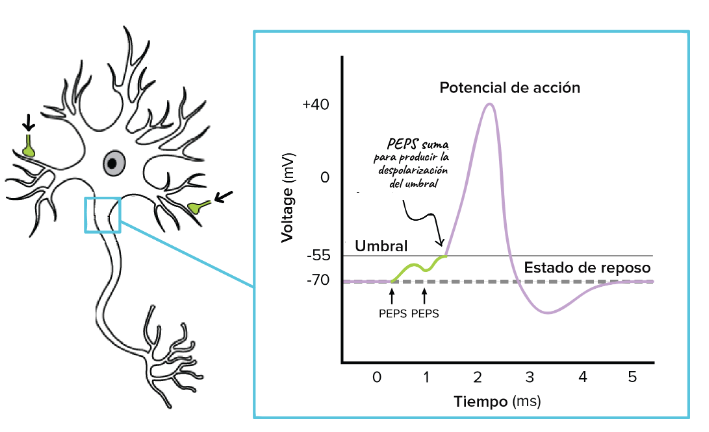
\includegraphics[width=12.0cm]{figures/PIPS_PEPS.png}
    \caption{Suma espacial de PEPS}
    \label{fig:suma_espacial_peps}
\end{figure}
Por otro lado, si ocurrió un PIPS junto con los dos PEPS, podría impedir que el potencial de membrana alcance el umbral y evita que la neurona dispare un potencial de acción. 
    \item La integración de potenciales postsinápticos que ocurren en el mismo lugar pero en momentos ligeramente diferentes se llama \textbf{suma temporal}. Ejemplo:\\
    Si una neurona presináptica se dispara rápidamente dos veces seguidas y causa dos PEPS, el segundo PEPS puede llegar antes que el primero se disipe\footnote{\footnotesize Los potenciales postsinápticos no son instantáneos; por el contrario, duran un ratito antes de disiparse}, lo que lleva el potencial de membrana hacia el umbral.
\end{itemize}
\section{Sinapsis eléctrica}
En las \textbf{sinapsis eléctricas} existe una conexión física directa entre la neurona presináptica y la neurona postsináptica. Esta conexión toma la forma de un canal llamado \textbf{unión de hendidura}, que permite que la corriente -los iones- fluyan directamente de una célula a otra (ver figura~\ref{fig:sinapsis_electrica}).Las sinapsis eléctricas transmiten señales con mayor velocidad que las sinapsis químicas.
\begin{figure}[htbp!]
    \centering
    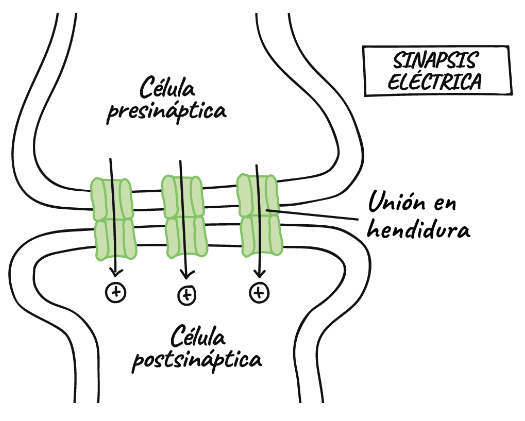
\includegraphics[width=6.5cm]{figures/Sinapsis_electrica.png}
    \caption{Sinapsis eléctrica}
    \label{fig:sinapsis_electrica}
\end{figure}

\chapter{Modelos de neurona}
Un \textit{modelo biológico de neurona} es una descripción matemática de las propiedades de ciertas células en el sistema nervioso, que genera potenciales eléctricos fuertemente marcados a través de la membrana de la célula, con una duración de unos pocos milisegundos (ver figura~\ref{fig:potencial_accion_real}).\\
Los modelos de neurona se pueden dividir en dos categorías, cada una de las cuales pueden seguir siendo subdivididas de acuerdo al nivel de abstracción y de detalle necesario.
\begin{enumerate}
    \item \emph{Modelos eléctricos de entrada-salida de voltaje de membrana}: Estos modelos realizan una predicción de los voltaje de salida en función de un estímulo eléctrico en la etapa de entrada (puede ser tanto voltaje o corriente). Algunos modelos en esta categoría son modelos de cajas negras y distinguen solo entre dos niveles de voltaje medidos, la presencia de un \textit{pico} (el potencial de acción) y un estado inactivo.
    \item \emph{Modelos de entrada natural o farmacológica}: Las entradas no son eléctricas sino que pueden ser farmacológicas (químicas) o físicas, caracterizadas por un estímulo externo como la luz, el sonido u otras formas de presión física. La salida representa la probabilidad de ocurrencia de un pico y no la producción de un voltaje de salida.
\end{enumerate}
En el campo de la ingeniería, interesan los modelos eléctricos de entrada-salida de voltaje, porque en esta categoría se describe la relación entre las corrientes de membrana de entrada y el voltaje de membrana de salida. Se pueden emplear elementos conocidos en ingeniería para modelar una neurona, como por ejemplo, capacitores, resistencias, fuentes de tensión y fuentes de corriente.
\newpage
\section{Electrónica básica y la neurona}
\subsection{Corriente eléctrica}
El fenómeno de la transferencia de carga desde un punto de un circuito a otro se describe mediante el término de \textit{corriente eléctrica}. La corriente eléctrica se puede definir como la rapidez con la que la carga eléctrica se transfiere a través de un corte transversal del conductor \cite{van1974network}.\\
Un movimiento desordenado de electrones dentro de un metal no constituye una corriente a menos que haya una transferencia neta de carga con el tiempo.\\
La corriente es:
\begin{equation}\label{eq:corriente_def}
    \tcbhighmath[boxrule=1pt,arc=1pt,colback=blue!10!white,colframe=black]{i=\dv{q}{t}}
\end{equation}
Cuando las neuronas transmiten impulsos, a través de sus membranas fluye corriente \cite{cnsclinicwebsite}. Esto quiere decir que existe una transferencia de carga, pero a diferencia de la transferencia de carga en un circuito eléctrico, donde la carga es la que aporta un electrón, en los sistemas biológicos, como la neurona, la carga la aporta un ion.\\
Como la neurona tiene concentración alta de $Na^+$ afuera y baja adentro (ver figura~\ref{fig:concentracion_iones}), la corriente circula desde afuera hacia adentro de la célula, atravesando la membrana. De manera similar, existen corrientes que van desde el interior hacia afuera de la célula debido al movimiento de los iones $k^+$ que se encuentran en mayor concentración adentro de la célula que afuera (ver figura~\ref{fig:corriente_membrana}).
\begin{figure}[htbp!]
    \centering
    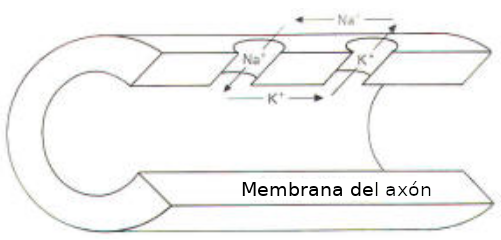
\includegraphics[width=7cm]{figures/corriente_membrana.png}
    \caption{Corriente a través de la membrana}
    \label{fig:corriente_membrana}
\end{figure}
\subsection{Resistencia y conductancia}\label{sec:resistencia_conductancia}
Todos los medios de conducción ofrecen algún grado de resistencia al paso de la corriente (indistintamente si es debido a la circulación de electrones o a la circulación de iones). La unidad de \textit{resistencia} R es el ohm ($\Omega$). El recíproco de la resistencia es la \textit{conductancia} g y su unidad es el siemens (S) aunque también se utiliza el término mho (ohm al revés) en la literatura clásica.
\begin{equation}
    \tcbhighmath[boxrule=1pt,arc=1pt,colback=blue!10!white,colframe=black]{g=\frac{1}{R}}
\end{equation}
Las membranas neuronales se comportan en parte como si estuvieran formadas por \textit{resistencias en paralelo} (fig.~\ref{fig:resistencia_fluidos}) mientras que los fluidos intracelulares y extracelulares que rodean a la membrana se comportan como \textit{resistencias en serie} (fig.~\ref{fig:resistencia_membrana}).
\begin{figure}[htbp!]
    \centering
    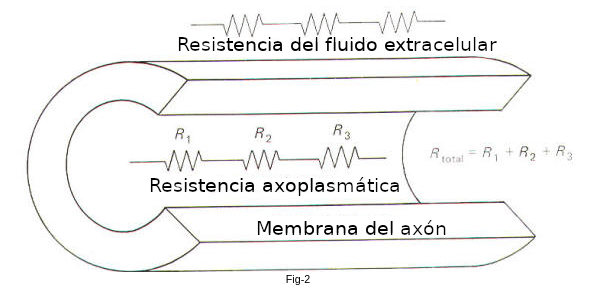
\includegraphics[width=9.0cm]{figures/Resistencia_Fluidos.png}
    \caption{Resistencia en serie del axoplasma y del fluido extracelular}
    \label{fig:resistencia_fluidos}
\end{figure}
La \textbf{\emph{resistencia de membrana}} representa la dificultad que tienen los iones en atravesarla a través sus respectivos canales. Su recíproco, \textbf{\emph{la conductancia}}, representa la facilidad que tienen los iones para atravesar la membrana.
\begin{figure}[htbp!]
            \centering 
            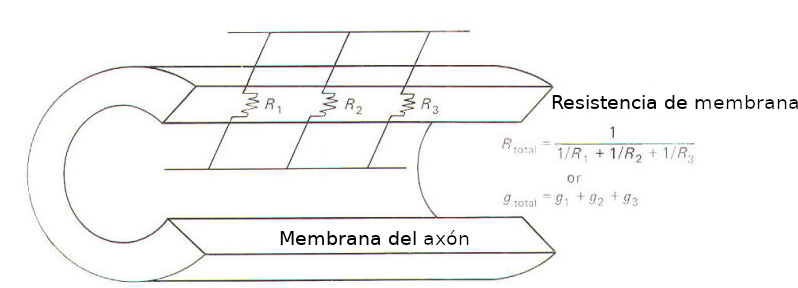
\includegraphics[width=11.0cm]{figures/Resistencia_Membrana.png}
            \caption{Membrana del axón en forma de resistencia en serie}
            \label{fig:resistencia_membrana}
\end{figure}

\subsection{Capacitancia}
 Un capacitor es un elemento que almacena energía en un campo eléctrico. Consiste en dos platos conductores separados por un dieléctrico y el mismo queda representado por un parámetro llamado \textit{capacitancia}:
\[C=\frac{\epsilon A}{d}\]
donde $\epsilon$ es la constante del dieléctrico, A es el área de los platos y d es la distancia que los separa. La unidad de la capacitancia es el \textit{faradio}.\\
La capacitancia es una medida de la habilidad que tiene un dispositivo para almacenar energía.\\
La carga almacenada por un capacitor es proporcional a su voltaje:
\[q= C.v\]
donde la constante de proporcionalidad C es la \textit{capacitancia} del capacitor.\\
La corriente se relaciona con la tensión mediante la ecuación diferencial:
\begin{equation}\label{eq:corriente_capacitor}
    \tcbhighmath[boxrule=1pt,arc=1pt,colback=blue!10!white,colframe=black]{i_c= C\dv{V}{t}}
\end{equation}
La membrana neuronal se comporta en parte como si estuviera compuesta por capacitores en paralelo (ver figura~\ref{fig:capacitores_paralelo_membrana}).
\begin{figure}[htbp!]
    \centering
    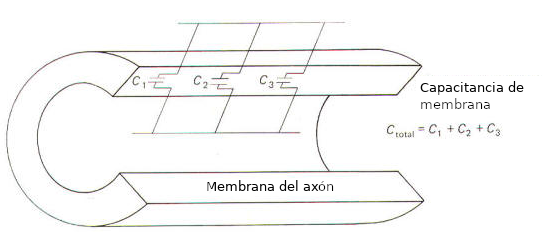
\includegraphics[width=9.0cm]{figures/capacitancia_membrana.png}
    \caption{Membrana como capacitores en paralelo}
    \label{fig:capacitores_paralelo_membrana}
\end{figure}
En la neurona, el interior de la membrana representa el dieléctrico, mientras que el fluido extracelular y el axoplasma representan los conductores (ver figura~\ref{fig:capacitor_membrana}).
\begin{figure}[htbp!]
    \centering
    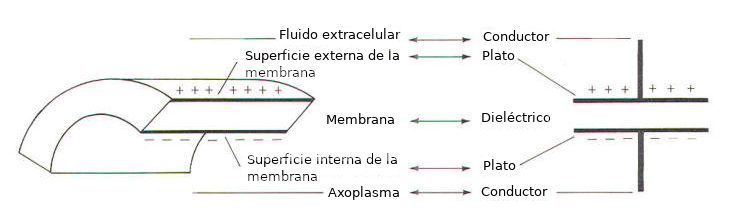
\includegraphics[width=11.5cm]{figures/dielectrico_neurona.png}
    \caption{Membrana como capacitor}
    \label{fig:capacitor_membrana}
\end{figure}
\textbf{\emph{La capacitancia de membrana representa la facilidad con que se carga la membrana}}
\subsection{Fuentes de tensión y de corriente}
La tensión eléctrica es la diferencia de potencial entre dos puntos. El voltaje a través de un elemento, es el trabajo (o la energía) requerido para mover una unidad de carga positiva desde la terminal negativa (-) hacia la terminal positiva (+). La unidad de voltaje es el volt (V). \cite{dorf2013introduction}.\\
Una fuente es un generador de tensión o de corriente, capaz de suministrar energía a un circuito. El generador de tensión es una fuente de carga (de electrones en circuitos eléctricos).\medskip \\ 
\textbf{\emph{En las neuronas, los iones representan la carga y el gradiente de concentración para un tipo de ion dado (ver~\ref{section:Potencial_Membrana}) representa la tensión de ese ion (el gradiente se puede representar mediante una fuente de tensión).}}\medskip \\
\textbf{\emph{La bomba sodio-potasio (ver~\ref{sec:bomba_sodio_potasio}) se puede representar mediante una fuente de corriente}}.
\begin{figure*}[htbp!]
        \centering
        \begin{subfigure}[b]{0.25\textwidth}
            \centering
            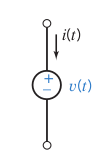
\includegraphics[width=2cm]{figures/fuente_tension.png}
            \caption{Fuente de tensión}
            \label{fig:fuente_tension}
        \end{subfigure}
       \hspace{0.5cm}
        \begin{subfigure}[b]{0.25\textwidth}  
            \centering 
            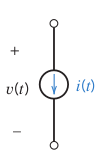
\includegraphics[width=2.0cm]{figures/fuente_corriente.png}
            \caption{Fuente de corriente}
            \label{fig:fuente_corriente}
        \end{subfigure}
        \quad
        \caption{Fuentes independientes}
        \label{fig:fuentes_independientes}
\end{figure*}
\section{Modelos eléctricos de entrada-salida}
La investigación más extensa realizada en esta categoría es la correspondiente al modelo de Hodking-Huxley \cite{HODGKIN1952}. En este modelo, el comportamiento eléctrico de la membrana puede ser representado por la red de la figura~\ref{fig:circuito_electrico_hodking_huxley}. 
\begin{figure}[htbp!]
    \centering
    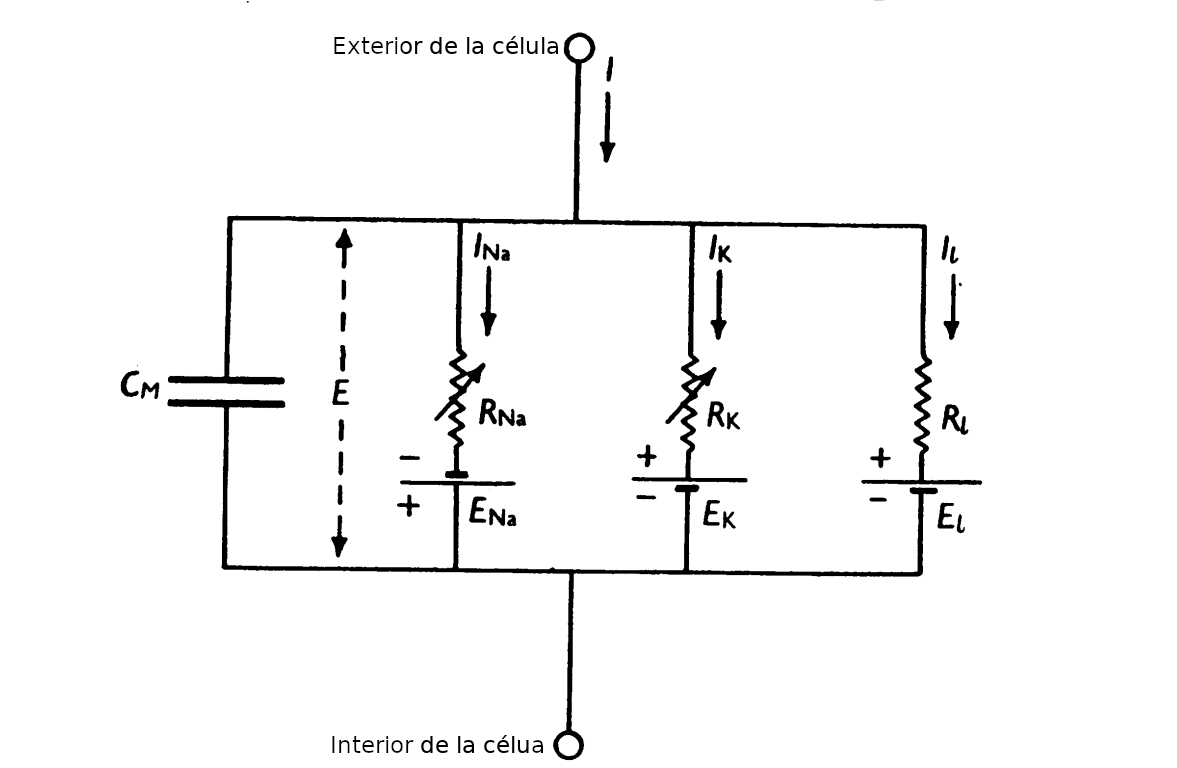
\includegraphics[width=10cm]{figures/Modelo_Hodking_Huxley+.png}
    \caption{Modelo de Hodgkin-Huxley. Circuto eléctrico que representa a una membrana. $R_{Na}=\frac{1}{g_{Na}}$, $R_{k}=\frac{1}{g_{k}}$, $R_{l}=\frac{1}{g_{l}}$. $R_{Na}$ y $R_k$ varían con el tiempo y el potencial de membrana. Los otros componentes son constantes}
    \label{fig:circuito_electrico_hodking_huxley}
\end{figure}
En el análisis realizado en \cite{HODGKIN1952}, se obtiene un conjunto de ecuaciones no lineales.
Existe una larga lista de modelos que derivan del modelo de Huxley-Hodgkin que tratan de simplificar la complejidad de las ecuaciones reduciendo el número de variables o los no linealidades asociadas. Uno de los objetivos es de reducir el cálculo computacional y permitir realizar simulaciones. En el presente trabajo se estudian modelos que derivan del \textit{integrate and fire}.
\subsection{Modelo Integrate and fire}
Es uno de los primeros modelos neuronales (1907). Se modela una neurona simplemente usando un capacitor (fig.~\ref{fig:integrate_and_fire}) y se plantea la ecuación~\ref{eq:corriente_capacitor} para determinar la corriente que circula por el mismo.
\begin{figure}[htbp!]
    \centering
    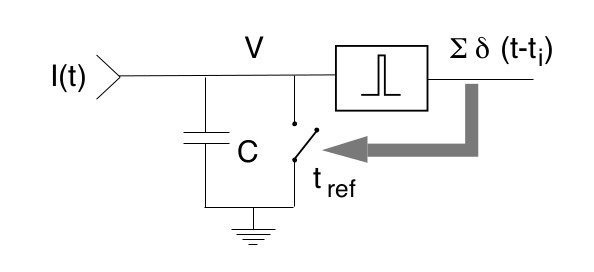
\includegraphics[width=10cm]{figures/prefect_integrate_and_fire.png}
    \caption{Integrate and fire}
    \label{fig:integrate_and_fire}
\end{figure}
Se caracteriza por tener un dominio de operación por debajo de un umbral y un voltaje umbral $v_{th}$ para la generación del impulso. El integrador perfecto, para lidiar con el modo de operación por debajo del umbral, utiliza simplemente un capacitor. Se asume que la corriente i(t) surge tanto desde una entrada sináptica como desde un electrodo intracelular.\\
La evolución del voltaje del integrador perfecto está gobernado por la ecuación diferencial de primer orden ~\ref{eq:corriente_capacitor}. Junto con la condición inicial, la ecuación~\ref{eq:corriente_capacitor} especifica la evolución en el tiempo del potencial de membrana durante la operación por debajo del umbral.\\
Una vez que el potencial llega a $v_th$, se dispara un impulso y el capacitor se conecta a tierra (cerrando la llave de la figura~\ref{fig:integrate_and_fire}) para descargar la carga que se había acumulado en el capacitor. Enviar la carga a tierra tiene el efecto instantáneo de resetear el potencial V(t) a cero. Se modela el potencial de acción asumiendo que en el instante t' en el cual $v(t')=v_{th}$, se genera un pulso de salida descrito por una función delta $\delta(t-t')$. Los tiempos sucesivos, $t_i$, de ocurrencia de un impulso se determinan recursivamente por la ecuación:
\[\int_{t_i}^{t_{i+1}} i(t) dt = C.v_{th}(t)\]
Una forma de caracterizar el comportamiento de la célula es mediante la relación entre la corriente inyectada y el promedio de la tasa de disparo (calculado como la inversa del intervalo entre impulsos).\\
En respuesta a una corriente aplicada en la entrada, el potencial de membrana va a cargar al capacitor hasta alcanzar $v_{th}$ y $v$ se resetea a 0 (cero). Cuanto mayor sea la corriente, menor va a ser el intervalo entre impulsos y más alta será el promedio de la tasa de disparo de acuerdo a:
\begin{equation}\label{eq:simple_firing_rate}
    <f>=\frac{i}{C.v_{th}}
\end{equation}
Hay unas cuestiones importantes que se desprenden de la ecuación~\ref{eq:simple_firing_rate}:
\begin{itemize}
    \item El promedio de la tasa de disparo depende linealmente de la corriente.
    \item Corrientes arbitrariamente pequeñas eventualmente van a producir un impulso, porque ninguna entrada se olvida. Cuando ingresa una corriente pequeña, esta corriente va a cargar al capacitor hasta una tensión determinada, menor a $v_{th}$. El capacitor va a mantener el valor de esa tensión (la va a recordar). A medida que ingresen más corrientes pequeñas que aporten una tensión menor a la umbral, estas tensiones se van a ir sumando hasta que en algún momento, la suma de todas ellas supere al umbral y produzca un disparo de un impulso.
    \item El tren de pulsos de salida es perfectamente regular. Las neuronas reales raramente, o nunca, responden a una corriente inyectada con un tren de pulsos espaciados de manera regular, sino que en realidad muestran una variabilidad en el tiempo entre impulsos (esto es lo que ocurre en el registro de neuronas \textit{in vivo}\cite{10.5555/1137840}).
\end{itemize}
El rango dinámico de la tasa de disparo de las células nerviosas está limitado por el hecho del que la corriente del sodio, responsable de la generación del impulso, se tiene que recuperar de la inactivación. Para simular el período refractario (sección~\ref{subsec:periodo_refractario}), hay que cerrar la llave de la figura~\ref{fig:integrate_and_fire} por un tiempo $t_{ref}$ determinado, poniendo en cero al potencial de membrana. Cualquier corriente que arribe durante ese tiempo va a ser desviada a tierra. Con esto se introduce una relación no lineal:
\begin{equation}
   \tcbhighmath[boxrule=1pt,arc=1pt,colback=blue!10!white,colframe=black]{ <f>=\frac{i}{C.v_{th}+t_{ref}.i}}
\end{equation}
La salida de este integrador frente a una entrada arbitraria de corriente consiste de una serie de impulsos $\sum_i \delta(t-t_i)$, todos espaciado al menos $t_{ref}$ entre sí. 
\newpage
\subsection{Modelo Leaky Integrate and fire}\label{sec:modelo_leaky_integrate_and_fire}
Para no tener la propiedad de \textit{memoria} y no recordar un valor de tensión no deseado, se agrega un término de fuga (\textit{leak}) al potencial de membrana. Este término refleja la difusión de iones cuando no se alcanza un estado de equilibrio en la célula.
\begin{figure}[htbp!]
    \centering
    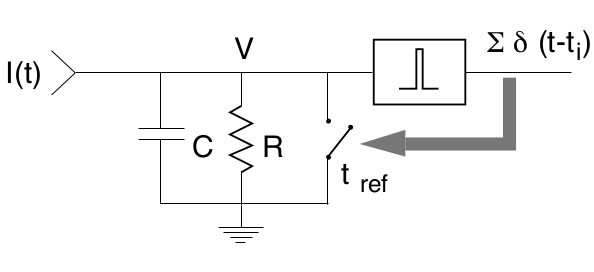
\includegraphics[width=10cm]{figures/leaky_integrate_and_fire.png}
    \caption{leaky Integrate and fire}
    \label{fig:leaky_integrate_and_fire}
\end{figure}
 El modelo \textit{leaky integrate and fire} tiene en cuenta esta fuga usando un circuito eléctrico formado por un capacitor y una resistencia en paralelo como se indica en la figura~\ref{fig:leaky_integrate_and_fire}.\\
Analizando la división de la corriente de entrada i(t), manteniendo la llave abierta (figura~\ref{fig:leaky_integrate_and_fire}), obtenemos:
\begin{equation}\label{eq:suma_corrientes_leaky}
    i(t)= i_R + i_C
\end{equation}
La corriente que atraviesa al capacitor ($i_c(t)$) es la que se indica en la ecuación~\ref{eq:corriente_capacitor}. La corriente que circula por la resistencia es:
\begin{equation}\label{eq:corriente_resistencia}
    \boxed{i_r(t)=\frac{v(t)}{R}}
\end{equation}
Reemplazando \ref{eq:corriente_capacitor} y \ref{eq:corriente_resistencia} en la ecuación~\ref{eq:corriente_resistencia},
\[
i(t)= C\dv{v}{t}+ \frac{v(t)}{R}
\]
Multiplicando por R:
\begin{equation}\label{eq:suma_corrientes_eq_diferencial_leaky}
    R.i(t)=RC \dv{v}{t} + v(t)
\end{equation}
La constante de tiempo del circuito es $\tau=RC$. Reemplazando RC por $\tau$ en la ecuación~\ref{eq:suma_corrientes_eq_diferencial_leaky}:
\begin{equation}\label{eq:ecuacion_diferencial_leaky}
    \tcbhighmath[boxrule=1pt,arc=1pt,colback=blue!10!white,colframe=black]{\tau \dv{v}{t} + v(t) = R.i(t)}
\end{equation}
\[\tcbhighmath[fuzzy halo=1mm with blue!50!white,arc=2pt,
  boxrule=0pt,frame hidden]{cond.\ inicial\ v(t=0)= 0}\]
\begin{center}
\begin{tabular}{ r l}
\footnotesize{donde,}&\\
 \footnotesize{$v(t)$:}& \footnotesize{es el potencial de membrana}\\ 
 \footnotesize{i(t)}:& \footnotesize{corriente de entrada.}\\
 \footnotesize{C:}& \footnotesize{capacitancia de membrana}\\
 \footnotesize{R}:& \footnotesize{resistencia de fuga (leak)}
\end{tabular}
\end{center}
En la versión general del modelo de neurona leaky integrate and fire se incorpora un \textit{período refractario} (ver secciones~\ref{subsec:fases_potencial_accion} y~\ref{subsec:periodo_refractario}):
\begin{enumerate}
    \item Si $v$ alcanza el valor umbral en un tiempo $t=T_{th}$, se interrumpe la dinámica de la ecuación~\ref{eq:ecuacion_diferencial_leaky} durante un tiempo refractario $t_{ref}$.
    \item Luego de un tiempo $T_{th}$+ $t_{ref}$ se reinicia la integración con la nueva condición inicial $v=0$.
\end{enumerate}
La ecuación~\ref{eq:ecuacion_diferencial_leaky} es una ecuación diferencial ordinaria\footnote{\textit{Ordinaria}: Se refiere a que la diferenciación se hace sólo con respecto a la variable independiente \textit{t}.}, de primer orden\footnote{\textit{Primer orden}: se refiere a que la derivada de orden mayor que se encuentra en la ecuación es la primera.}, lineal\footnote{\textit{Lineal} significa que la variable independiente y sus derivadas aparecen sólo como términos de primer grado, es decir, no hay términos del tipo $v^2(t)$ o $v(t).\dv{v}{t}$ (estos dos términos son de segundo grado).}, no homogénea\footnote{\footnotesize \textit{No homogénea}: significa que la ecuación incluye un término como g(t) donde g(t) puede ser una constante o alguna función conocida de t.} y de coeficientes constantes\footnote{\textit{Coeficientes constantes} significa que los coeficientes C y 1/R son constantes, es decir, no son funciones de la variable \textit{t}.}. Este sistema es un \textit{filtro pasabajos} (ver sección~\ref{sec:filtro_pasabajos_primer_orden}). \\
Si se aplica una corriente constante en forma de escalón (ver sección~\ref{sec:respuesta_escalon}), conectada en t=0 y permaneciendo igual de forma constante de ahí en adelante, la respuesta a esta entrada es la indicada en la ecuación~\ref{eq:respuesta_escalon_leaky_integrator}. En la misma se puede observar que la membrana se carga exponencialmente hasta su valor estacionario $v=i.R$. Sin embargo, el modelo integrate and fire sólo sigue esta ecuación siempre que el voltaje este por debajo la tensión umbral $v_{th}$. Una vez que se alcanza el umbral, se genera un impulso y la tensión se resetea a 0 (cero).\\
La corriente mínima necesaria para disparar un potencial de acción (corriente umbral) es:
\[i_{th}=\frac{v_{th}}{R}\]
Para cualquier corriente i mayor que $i_{th}$ se va a generar un pulso de salida en el instante $T_{th}$ tal que se mantenga el valor $v_{th}=i.R.\big(1-e^{-\frac{T_{th}}{\tau}}\big)$. Despejando $T_{th}$:
\[\frac{v_{th}}{i.R}=1-e^{-\frac{T_{th}}{\tau}}\]
\[\frac{v_{th}}{i.R}-1=-e^{-\frac{T_{th}}{\tau}}\]
\[1-\frac{v_{th}}{i.R}=e^{-\frac{T_{th}}{\tau}}\]
\[\ln{\Big(1-\frac{v_{th}}{i.R}\Big)}=-\frac{T_{th}}{\tau}\]
\begin{equation}
    \tcbhighmath[fuzzy halo=1mm with blue!50!white,arc=2pt,
  boxrule=0pt,frame hidden]{T_{th}=-\tau.\ln{\Big(1-\frac{v_{th}}{i.R}\Big)}}
\end{equation}
Como el voltaje se resetea después de un impulso y asumiendo que la corriente de entrada persiste, la membrana se va a cargar hasta el umbral, generando el siguiente impulso un tiempo $T_{th}+t_{ref}$ después. El promedio de la tasa de disparo es:
\begin{equation}
   \tcbhighmath[boxrule=1pt,arc=1pt,colback=blue!10!white,colframe=black]{ <f>=\frac{1}{t_{ref}+T_{th}}=\frac{1}{t_{ref}-\tau.\ln{\Big(1-\frac{v_{th}}{i.R}\Big)}}}
\end{equation}

\chapter{Conceptos electrónicos}
\section{Filtro pasabajos de primer orden}\label{sec:filtro_pasabajos_primer_orden}
Aplicando la transformada de Laplace \cite{10.5555/248702} a la ecuación~\ref{eq:ecuacion_diferencial_leaky}, se obtiene:
\[
     \tau.\big(s .V(s) + v(0^-)\big) + V(s)= I(s)
\]
como la condición inicial es $v(0^-)=0$
\[
     \tau.s .V(s) + V(s)= R.I(s)
\]
\[
    V(s).\big( \tau.s + 1\big) = R.I(s)
\]
Finalmente se obtiene la \textit{función transferencia} del circuito, definida como el cociente entre la señal de salida y la señal de entrada:
\begin{equation}\label{eq:respuesta_en_frecuencia_filtro_RC}
     \tcbhighmath[boxrule=1pt,arc=1pt,colback=blue!10!white,colframe=black]{H(s)=\frac{V(s)}{I(s)} = \frac{R}{(\tau.s+ 1)}=\frac{1}{c}.\frac{1}{(s+\frac{1}{\tau})}}
\end{equation}
con la región de convergencia ROC=\big\{$\Re{s}>-\frac{1}{\tau}$\}\big.
Aplicando la transformada inversa de Laplace, se obtiene la respuesta al impulso:
\[
\tcbhighmath[fuzzy halo=1mm with blue!50!white,arc=2pt,
  boxrule=0pt,frame hidden]{h(t)= \frac{1}{c}.e^{-\frac{1}{\tau}.t}.u(t)}
\]
La ecuación~\ref{eq:respuesta_en_frecuencia_filtro_RC} es la función transferencia de un \textit{filtro pasabajos} \cite{dorf2013introduction}.
Como el sistema está descrito por una ecuación diferencial lineal, de coeficientes constantes (ver ecuación ~\ref{eq:ecuacion_diferencial_leaky}) y tiene condición inicial nula, dicho sistema es LTI. Se trata entonces, de un sistema de primer orden, lineal\footnote{Un elemento es \textit{lineal} si cumple con la propiedad de superposición, es decir, si $i_1$ produce la salida $v_1$ e $i_2$ produce la salida $v_2$ entonces la entrada $i_1+i_2$ produce la salida $v_1+v_2$; y si cumple con la propiedad de homogeneidad, es decir, si una entrada i produce una salida v, entonces al multiplicar por una constante a la entrada (k.i) produce como salida k.v} e invariante en el tiempo\footnote{Sistema invariante en el tiempo significa un corrimiento de tiempo en la señal de entrada produce un corrimiento de tiempo en la señal de salida. Si la salida y(t) corresponde a la entrada x(t), un sistema invariante en el tiempo tendrá una salida y($t-t_0$) para una entrada $x(t-t_0$)} \cite{10.5555/248702}.
\newpage
\subsubsection{Respuesta al escalón}\label{sec:respuesta_escalon}
Tomando como entrada $i(t)=i_0.u(t)$ (la entrada es la función escalón de altura $i_0$), se busca a continuación la tensión de salida correspondiente (respuesta al escalón).\\
La transformada de Laplace de la respuesta al escalón es\cite{10.5555/248702}:
\[V_{esc}(s)=H(s).I(s)=H(s).\frac{i_0}{s}=\]
\[=\frac{1}{c}.\frac{1}{\big(s+\frac{1}{\tau}\big)} . \frac{i_0}{s}=\]
\[= \frac{i_0}{c}.\Bigg[\frac{\tau}{s}-\frac{\tau}{(s+\frac{1}{\tau})}\Bigg]\]
\[con\ ROC=\big\{\Re{s}>0\big\}\]
Aplicando la transformada inversa de Laplace\cite{10.5555/248702}:
\[v_{esc}(t)=\frac{i_0}{c}.\Bigg[\tau.u(t)-\tau.e^{-\frac{t}{\tau}}.u(t)\Bigg]=\]
\[=\frac{i_0}{c}.\tau.[1-e^{-\frac{t}{\tau}}].u(t)\]
entonces la respuesta al escalón es: 
\begin{equation}\label{eq:respuesta_escalon_leaky_integrator}
    \tcbhighmath[boxrule=1pt,arc=1pt,colback=blue!10!white,colframe=black]{v_{esc}(t)=i_0.R.[1-e^{-\frac{t}{\tau}}].u(t)}
\end{equation}

\printbibliography[
    heading=bibintoc,
    title={Referencia completa}
]
\clearpage
\printbibliography[heading=subbibintoc,type=article,title={Referencias a artículos}]
\printbibliography[heading=subbibintoc,type=book,title={Referencias a libros}]
\printbibliography[heading=subbibintoc,type=online,title={Referencias en línea}]
\end{document}
